% =======================================================================
% Architecture globale Nova AI -- vue verticale en 3 couches
% =======================================================================
% Source : figures/sources/nova-archi.mmd (Mermaid)
% Image generee verticale (portrait), taille reduite pour partager la
% page avec le texte descriptif.
% =======================================================================
\begin{figure}[!htbp]\centering
\IfFileExists{figures/nova-archi.png}{%
  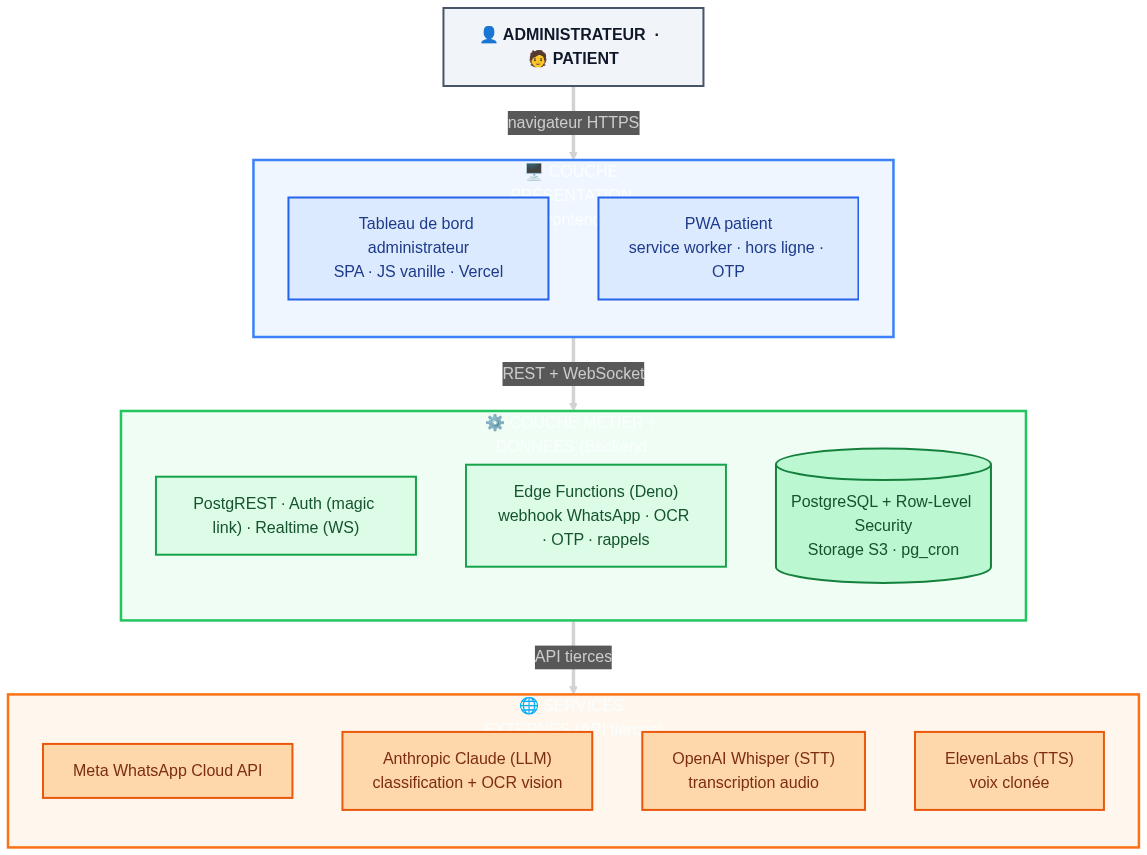
\includegraphics[width=.72\textwidth,height=1.0\textheight,keepaspectratio]{figures/nova-archi.png}%
}{%
  \fbox{\parbox[c][8cm][c]{0.42\textwidth}{\centering\itshape\small
    [Architecture globale (vue verticale) -- a generer depuis\\
    \texttt{figures/sources/nova-archi.mmd} via\\
    \url{https://mermaid.live} puis sauvegarder en\\
    \texttt{figures/nova-archi.png}]
  }}%
}
\caption{Architecture globale de \nova{} : trois couches empilées verticalement -- frontends, backend Supabase, services externes.}
\label{fig:nova-archi}
\end{figure}
